\documentclass[12pt]{article} 
\usepackage[left=2.5cm, right=2cm, top=2cm, bottom=2cm]{geometry} 
\usepackage{graphicx}
\usepackage[pages=some]{background}
\usepackage{titling}
\usepackage{tabularx}
\usepackage{tikz}
\usepackage{subfigure}
\usepackage{textcase}
\usepackage{newtxtext}
\usepackage{enumitem}
\usepackage{fancyhdr}
\usepackage{graphicx}

\pagestyle{fancy}
\fancyhf{} 
\renewcommand{\headrulewidth}{0pt} 
\rhead{\#1810009}

\begin{document}


  \subsection*{Experiment no: 2(a)}
  \subsubsection*{Experiment Name: Performance Test of a Centrifugal Pump} 
  \vspace*{0.3cm}
  \subsection*{Objectives:}
  To study the performance characteristics of the pump at constant speed when varying the flowrate. 
  \vspace*{0.3cm}
  \subsection*{Apparatus:}
  \begin{enumerate}
    \item Pressure gage
    \item Manometer 
    \item Wattmeter
    \item Tachometer 
    \item Scale \& Stopwatch 
  \end{enumerate}  
  
  \vspace*{0.3cm}

  \subsection*{Schematic Diagram:}
  \begin{figure}[h]
    \begin{center}
      \includegraphics*[width=0.80\linewidth]{img/schematic.jpeg}
      \caption{Schematic Diagram of Centrifugal Pump Test Rig.}
    \end{center}
  \end{figure}
\pagebreak
\subsection*{Discussion:}
In this experiment, we observed the results obtained from the performance test conducted on a centrifugal pump and analyze its characteristics based on the collected data. The performance test involved measuring various parameters such as flow rate, head, power consumption, and efficiency of the centrifugal pump under different operating conditions. These parameters provide insights into the pump's performance and its ability to handle fluid flow effectively.\\

One of the key point during the test was the pump's characteristic curve, which represents the relationship between the flow rate and head. By plotting the data points obtained from the test, we were able to observe the pump's behavior and determine its operating range. The characteristic curve helps in understanding the pump's efficiency and performance under different flow conditions.\\ 

One of the most crucial aspect analyzed during the performance test was the pump's efficiency. By calculating the efficiency at various operating points, we were able to determine the pump's efficiency curve. It was observed that the pump operated most efficiently within a specific flow rate range. Efficiency is decreased at both lower and higher flow rates. This behavior is because of internal losses and friction within the pump system.\\

The same scenario also observed for input power and output power. They increase upto a certain flow rate. After a threshold, both input and output power decresed. From the graph, it is also observed that, head is gradually decreasing with flow rate. There may be many reasons for that. For examplle - Viscous loss, Frictional loss,  flow separation, backflow, or other flow instabilities etc. \\

From the graph, the efficiency ($\eta$) was found maximum when flow rate ($Q$) = 0.004527 $m^3/s$. At that point,
\begin{center}
  The efficiency,$\eta$ = 57.17\% \\
  The Head, $H$ = 16.01 m \\
  The input power, $P_i$ = 1282.92 watt \\
  The output power, $P_o$ = 715.58 watt \\ 
\end{center}

Several factors can influence the performance of a centrifugal pump, including the condition of the impeller, impeller diameter, pump speed, and operating conditions. These factors can significantly impact the pump's efficiency and overall performance. By taking proper steps, some errors can be mitigated. 
\pagebreak
\subsection*{Answer to the Question}
\hspace*{0.5cm} \textbf{1) What do you understand by characteristics curve of centrifugal pump?}\\
Ans: The characteristic curve of a centrifugal pump shows the relationship between its head (pressure), efficiencey, power consumption with flow rate. It provides a visual representation of how the pump performs at different operating conditions, helping to understand its efficiency and performance capabilities.


\vspace*{.5cm}
\textbf{2) Decribe what is priming?}\\
Ans : Priming in a centrifugal pump is the process of removing air or gas from the pump to create a vacuum and enable efficient pumping of liquid. It ensures proper pump performance and prevents issues like loss of suction or cavitation.

\vspace*{.5cm}

\textbf{3) What is: NPSHA, NPSHR, cavitation?}\\
Ans: NPSHA (Net Positive Suction Head Available) is a measure of the total energy available at the suction side of a pump to overcome the pressure drop and prevent cavitation. It takes into account factors such as the pressure at the pump suction, the velocity of the fluid, and the elevation difference between the fluid source and the pump.\\

NPSHR (Net Positive Suction Head Required) is the minimum amount of NPSHA that a pump needs to operate without experiencing cavitation. It represents the pressure head necessary to prevent the formation of vapor bubbles and maintain proper pump performance.\\

Cavitation is a phenomenon that occurs when the pressure of a fluid drops below its vapor pressure, causing the formation and subsequent collapse of vapor bubbles within the pump. The collapsing bubbles create localized high-pressure zones, leading to pitting, erosion, and damage to the pump impeller and other components. Cavitation can significantly reduce pump efficiency, increase noise levels, and ultimately may cause mechanical failure.

\pagebreak
\subsection*{Experiment no: 2(b)}
\subsubsection*{Experiment Name: Experiment Name: Study of Centrifugal Pumps in Series and Parallel Connection} 

\vspace*{.5cm}
\subsubsection*{Objectives:}
To study the flow rate and head characteristics of two centrifugal pumps in series and parallel connections. 
\subsubsection*{Apparatus:}
  (a) Centrifugal Pump, 
  (b) Manometer, 
  (c) Valves, 
  (d) Pressure gage 

\subsubsection*{Schematic Diagram (Connection Circuit):}
\begin{figure}[h]
  \subfigure[Pump 2 off and Pump 1 running]{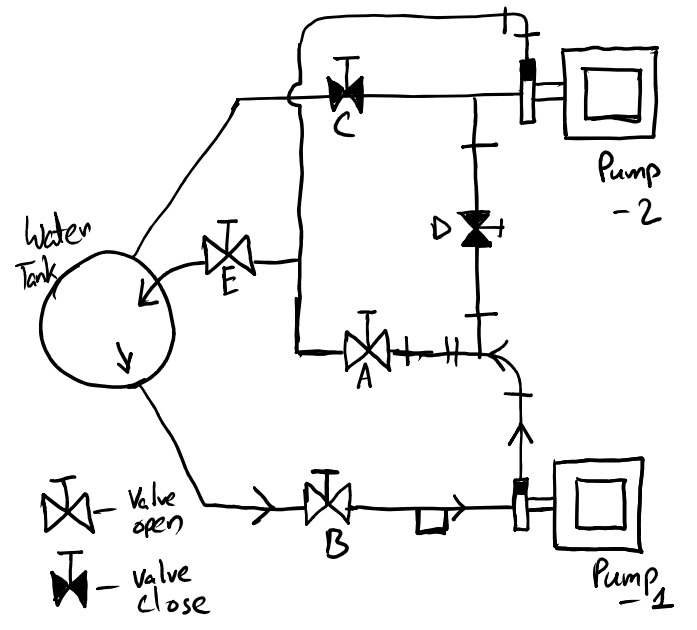
\includegraphics[width=0.40\linewidth]{img/1st_open_2nd_off.jpeg}}
  \hfill
  \subfigure[Pump 1 off and Pump 2 running]{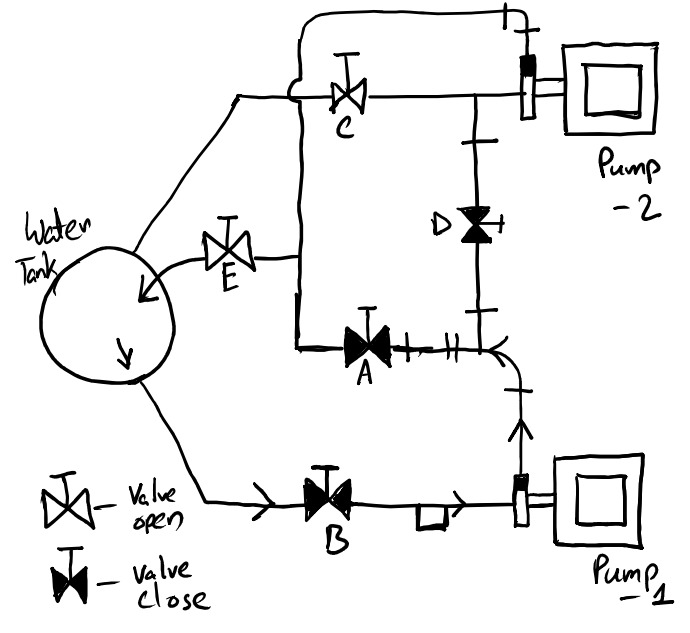
\includegraphics[width=0.40\linewidth]{img/1st_off_2nd_on.jpeg}}
  \hfill
  \subfigure[Both pumps in series connection]{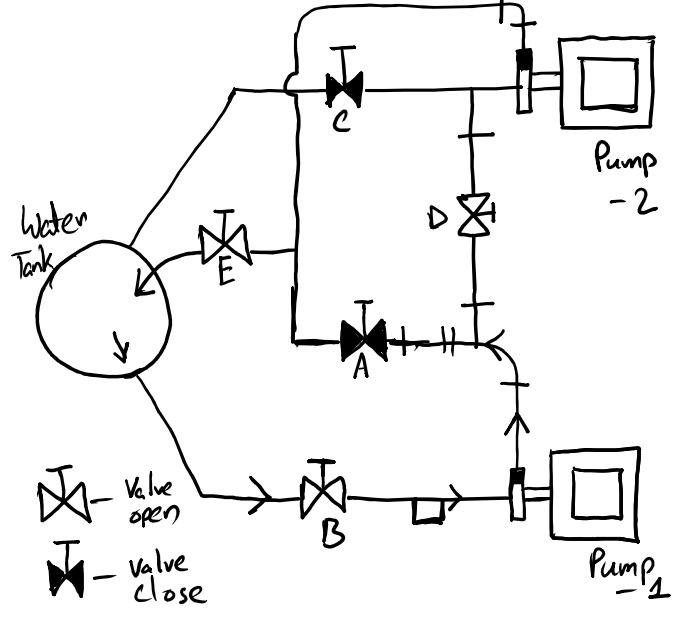
\includegraphics[width=0.40\linewidth]{img/series.jpeg}}
  \hfill
  \subfigure[Both pumps in parallel connection]{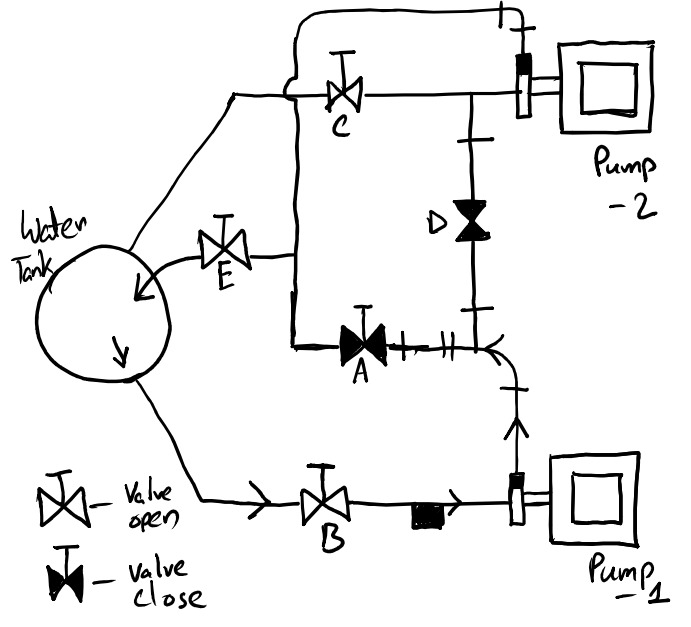
\includegraphics[width=0.40\linewidth]{img/parallel.jpeg}}
  \hfill

  % \vspace{0.2cm}


  % \vspace{0.2cm}
  \caption{Schematic Diagram (Connection Circuit)}
\end{figure}
\pagebreak

\begin{figure}[h]
  \begin{center}
    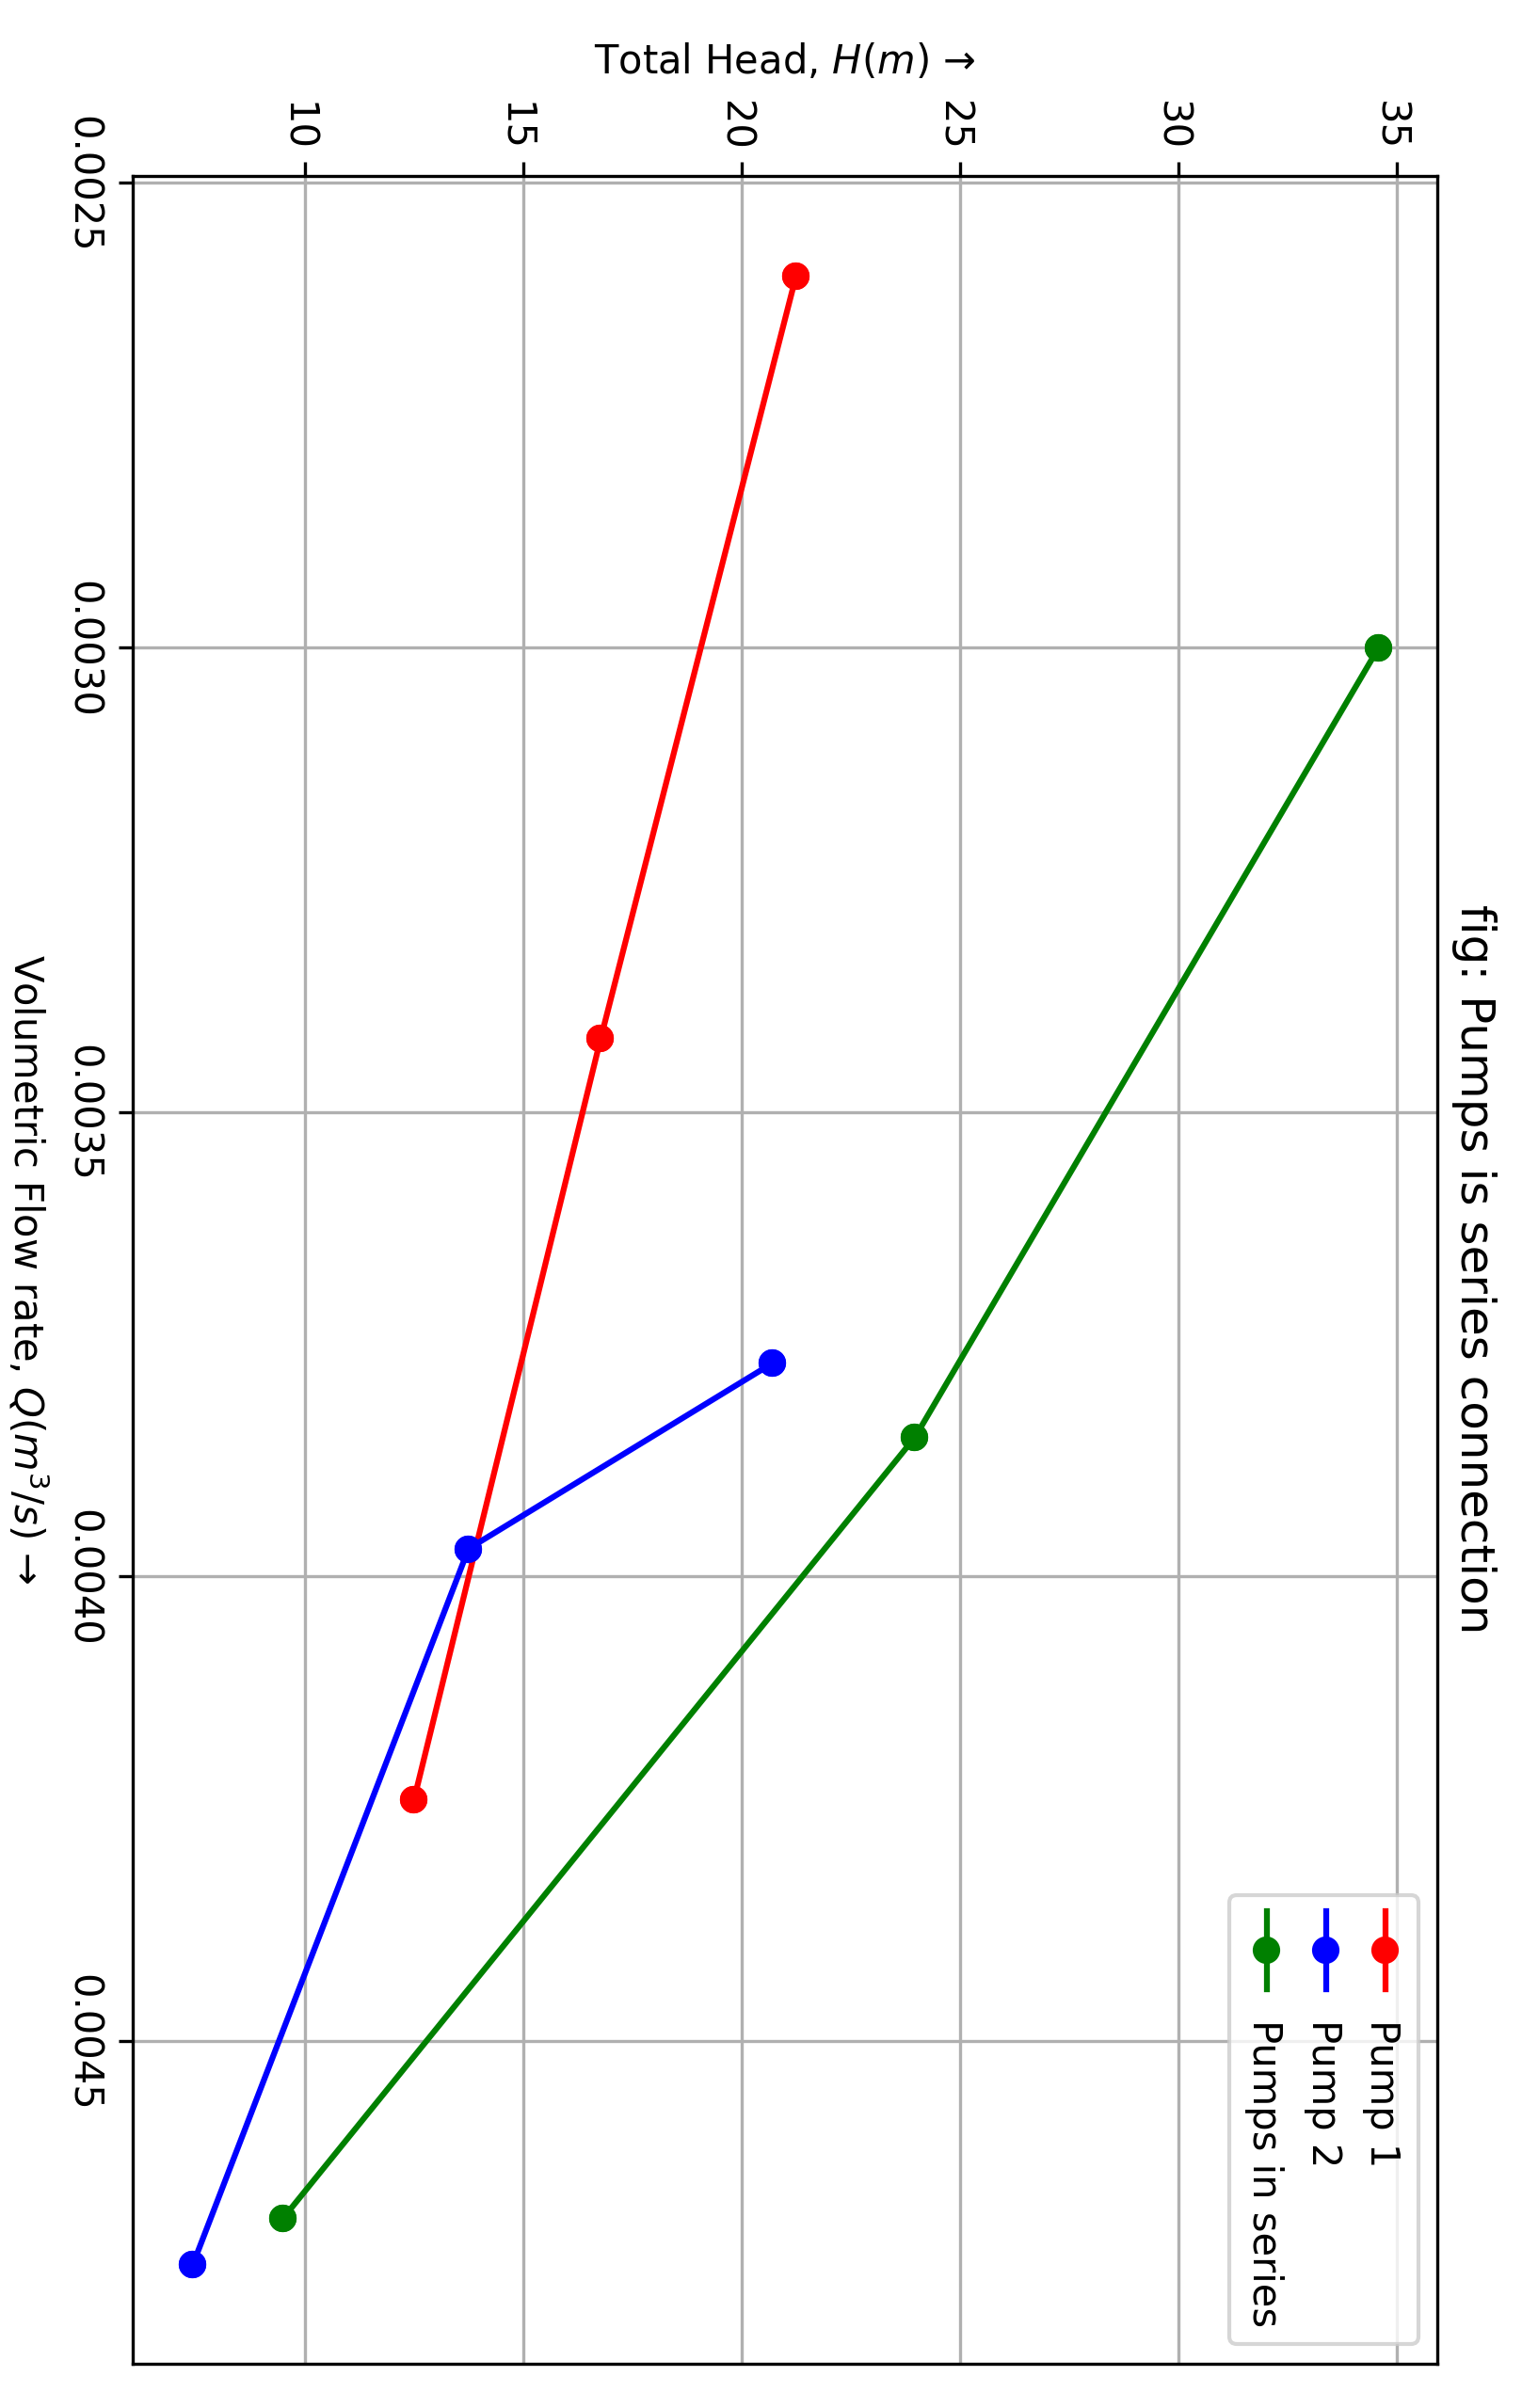
\includegraphics[width=0.85\linewidth]{img/series_graph.png}
  \end{center}
\end{figure}

\begin{figure}[h]
  \begin{center}
    
    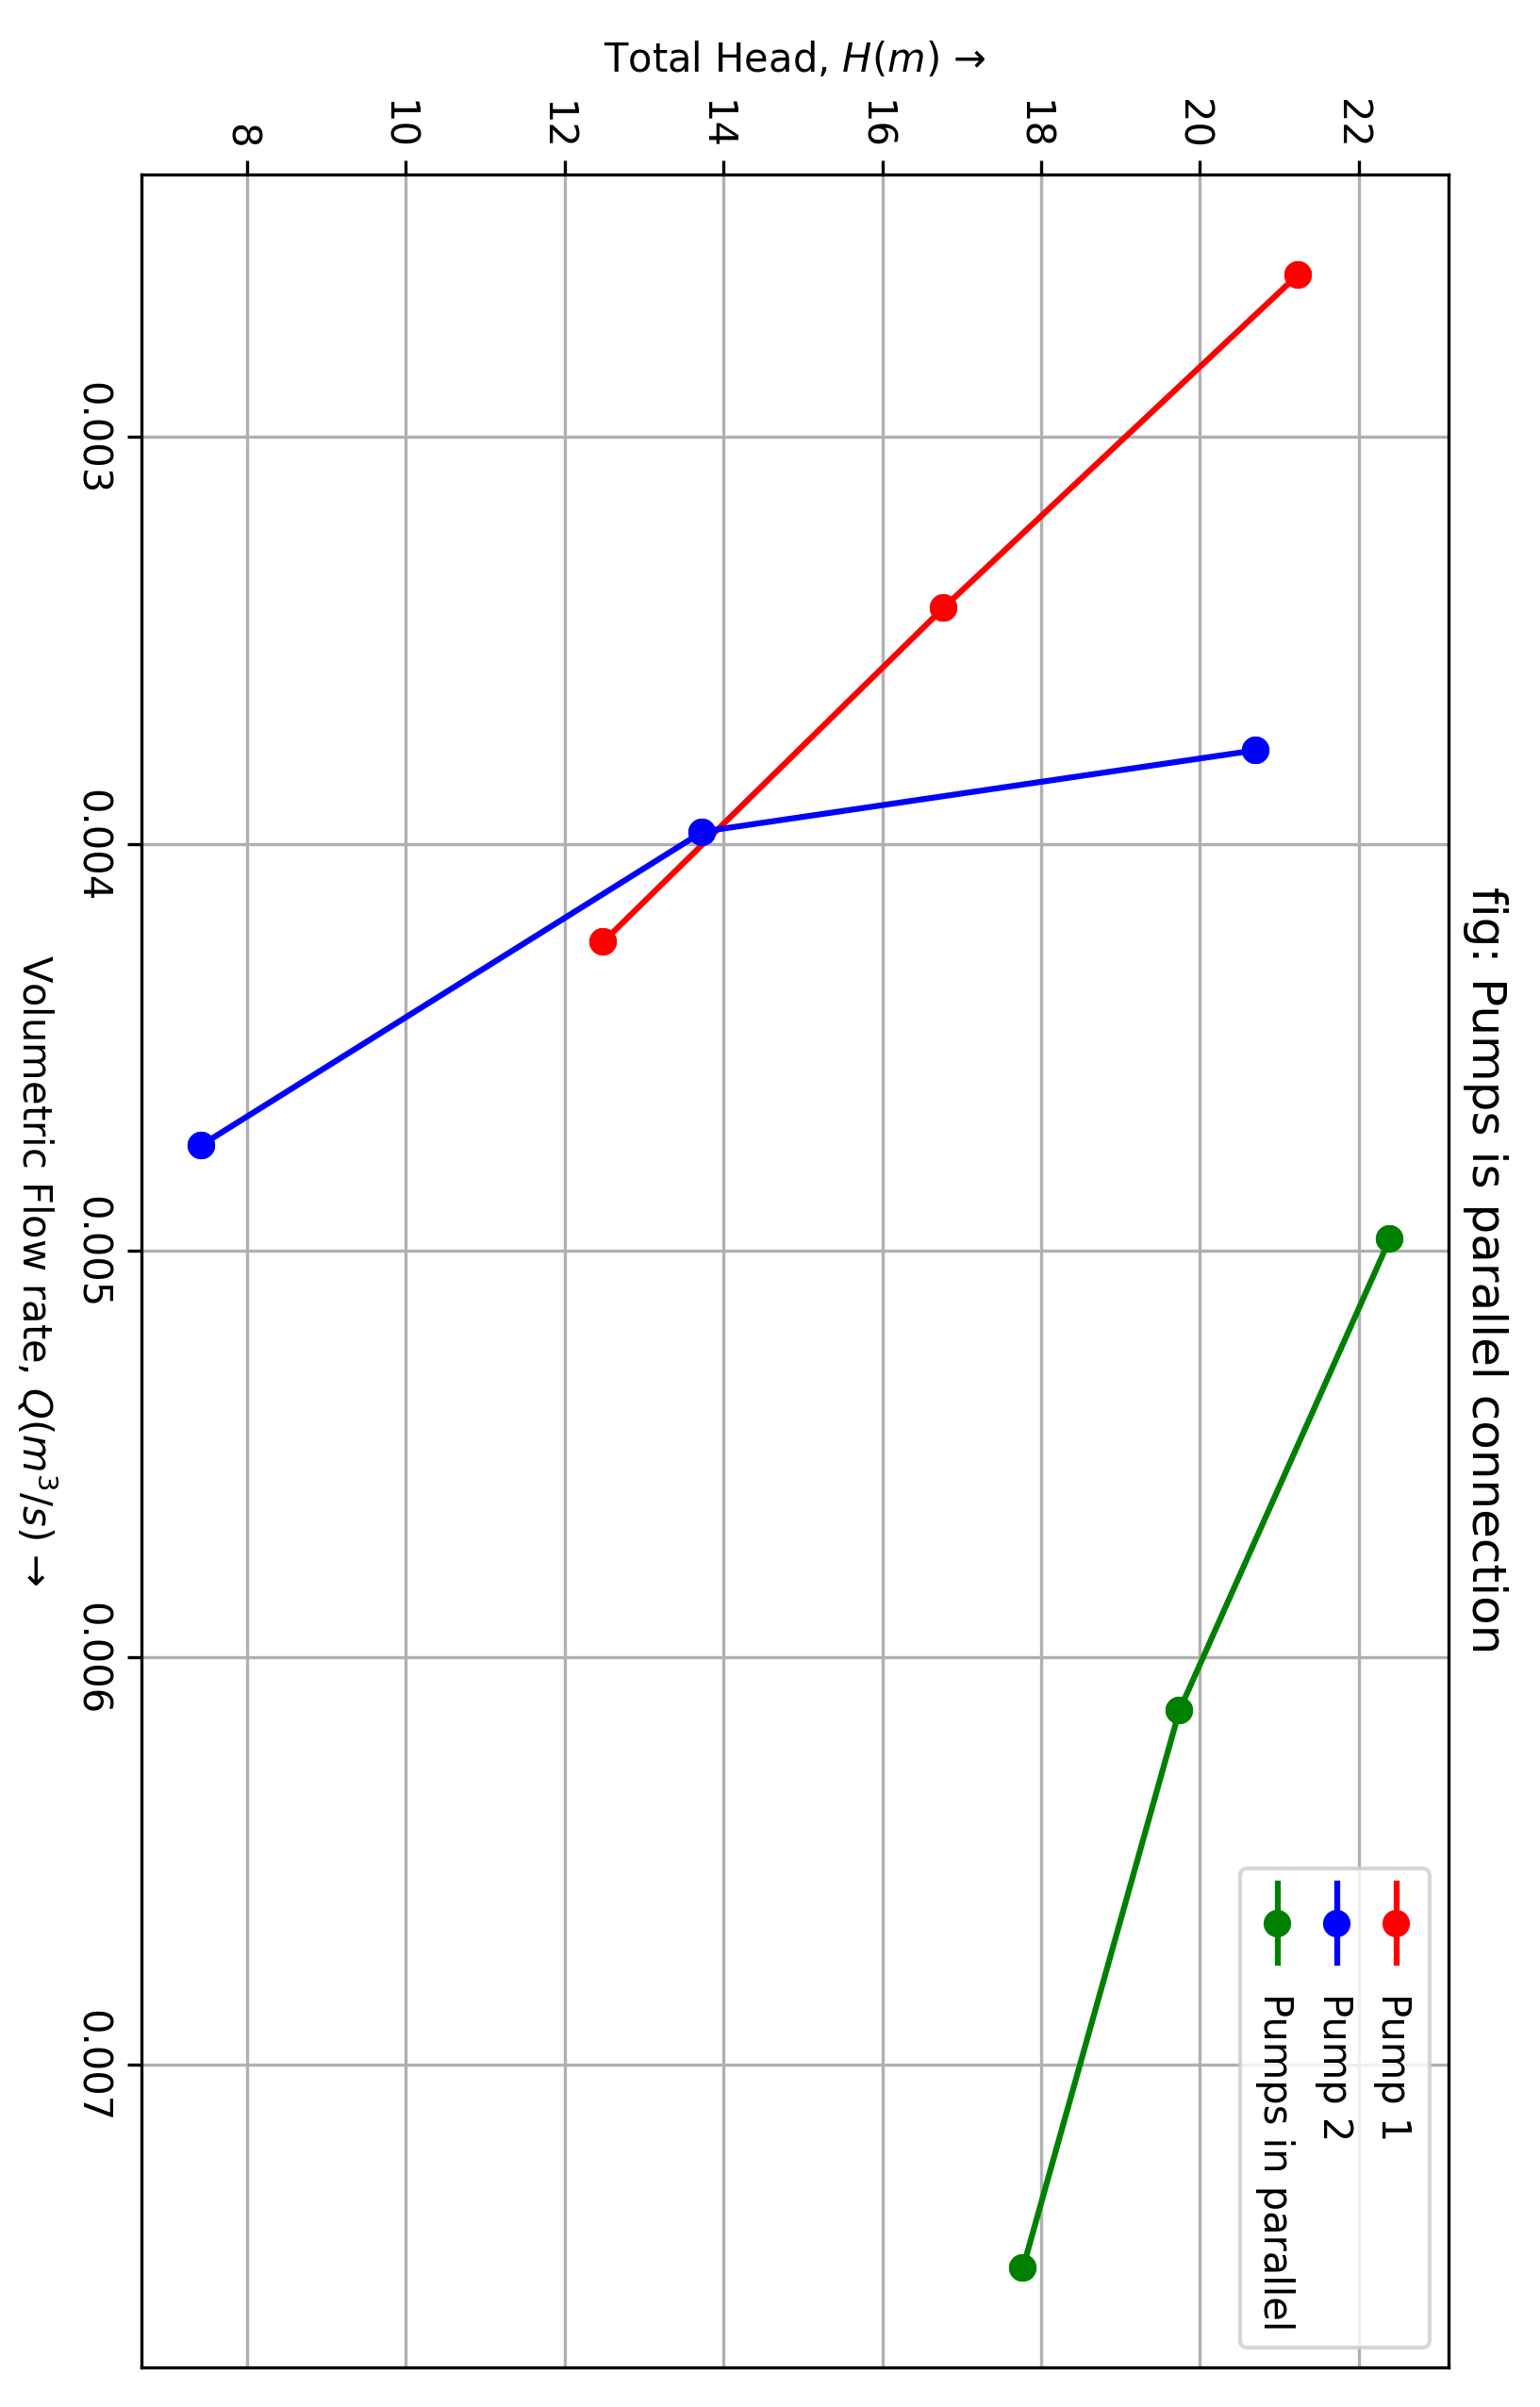
\includegraphics[width=0.85\linewidth]{img/parallel_graph.png}
  \end{center}
  \end{figure}

  \begin{figure}[h]
  \begin{center}
    
    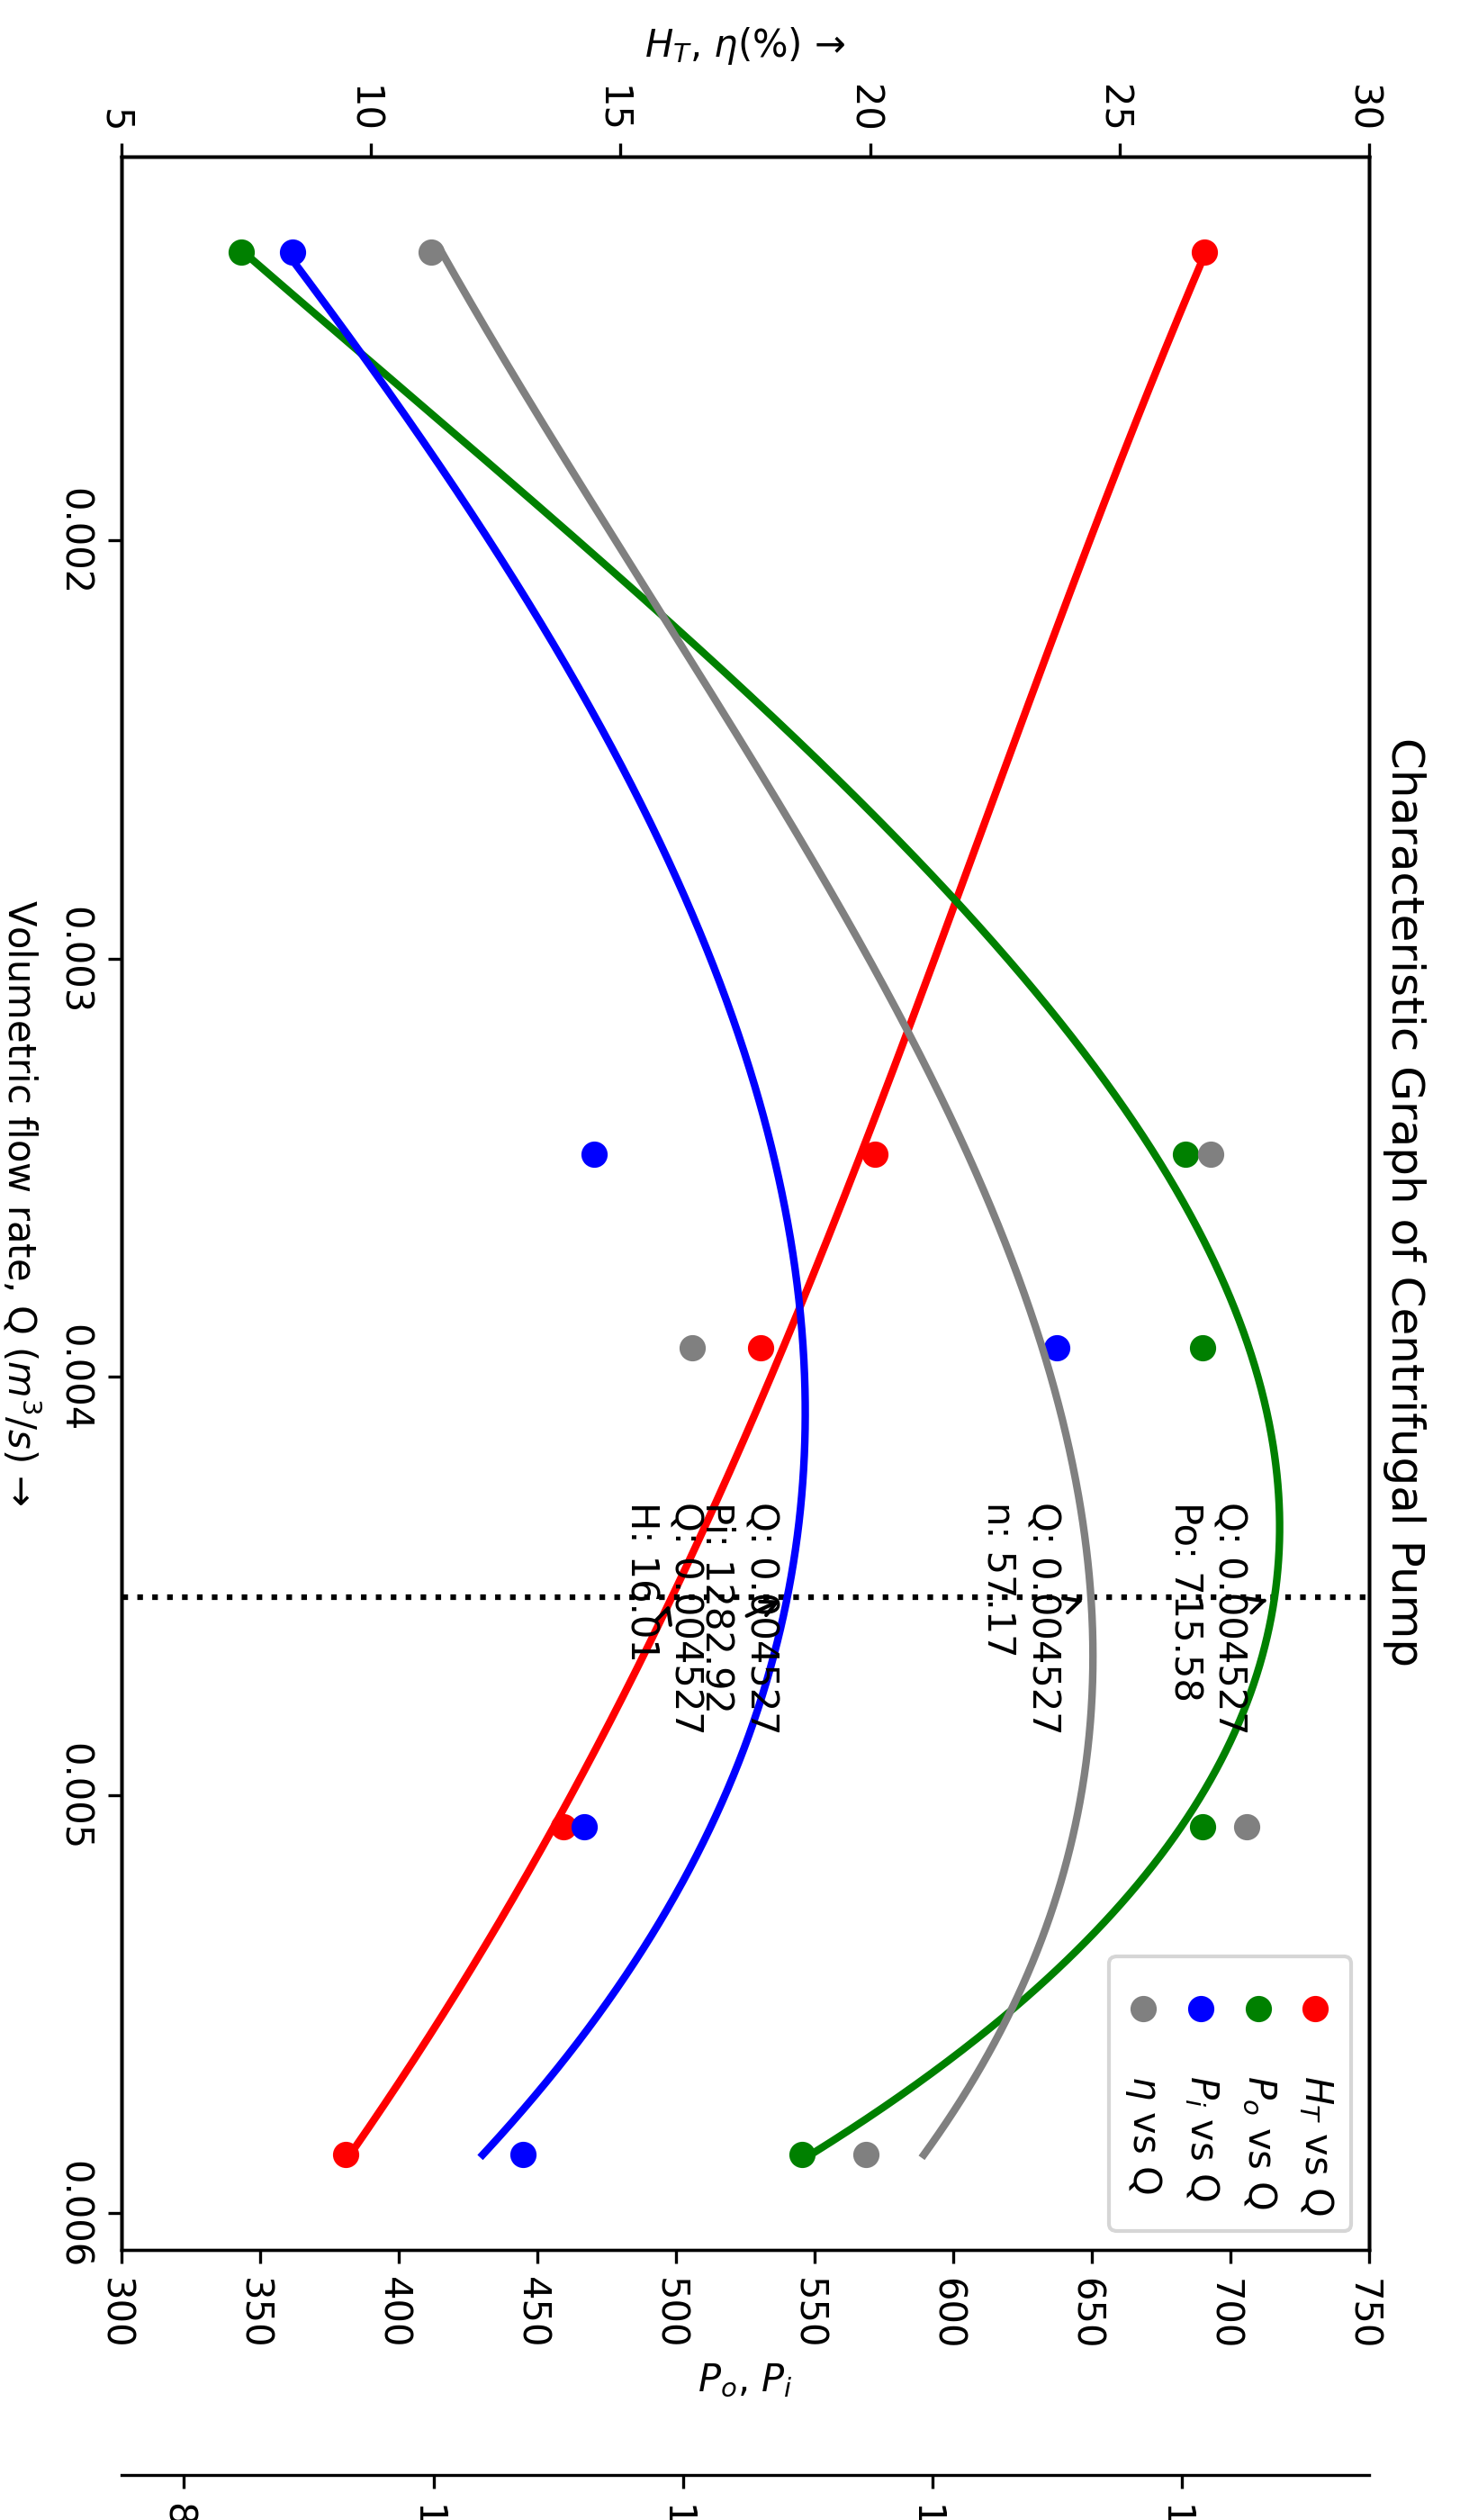
\includegraphics[width=0.85\linewidth]{img/characteriestics_graph.png}
  \end{center}
  \end{figure}

\pagebreak
\subsection*{Discussion:}
The experiment demonstrated the effects of connecting centrifugal pumps in series and parallel configurations. In series connection, the total head increased while maintaining a constant flow rate. This configuration is useful for applications where higher pressures are required. In parallel connection, the flow rate increased while maintaining a constant head. This configuration is beneficial for applications that demand higher flow rates. \\ 

The observed result experimentally has some deviation from theoretical or expected result, due to loss in the piping and fittings. Also the experimental results could be influenced by various factors, including pump characteristics, piping design, and measurement errors. To ensure accurate analysis and draw reliable conclusions, careful calibration of instruments and consideration of uncertainties are essential. 

\pagebreak
 
\end{document}
